%%% License: Creative Commons Attribution Share Alike 4.0 (see https://creativecommons.org/licenses/by-sa/4.0/)
%%% Slides are based heavily on earlier versions of this course taught by Jesper Rudiger.

\documentclass[english,10pt]{beamer}
\DeclareGraphicsExtensions{.eps, .pdf,.png,.jpg,.mps,}
\usetheme{reMedian}
\usepackage{parskip}
\makeatother

\renewcommand{\baselinestretch}{1.2} 

\usepackage{amsmath, amssymb, amsfonts, amsthm}
\usepackage{enumerate}
\usepackage{hyperref}
\usepackage{url}
\usepackage{bbm}
\usepackage{color}

\usepackage{tikz}
\usepackage{tikzscale}
\newcommand*\circled[1]{\tikz[baseline=(char.base)]{
\node[shape=circle,draw, inner sep=-20pt] (char) {#1};}}
\usetikzlibrary{automata,positioning}
\usetikzlibrary{decorations.pathreplacing}
\usepackage{pgfplots}
\usepgfplotslibrary{fillbetween}
\usepackage{graphicx}

\usepackage{setspace}
\thinmuskip=1mu
\medmuskip=1mu 
\thickmuskip=1mu 

\theoremstyle{definition} 
\newtheorem{thm}{Theorem}
\newtheorem{claim}{Claim}
\newtheorem{proposition}{Proposition}
\usecolortheme{default}
\usepackage{verbatim}
\usepackage[normalem]{ulem}
\usepackage{appendixnumberbeamer}



\title{Financial Markets Microstructure \\ Exercise class 1}

%\subtitle{Introduction and institutions \\
%Chapters 0 and 1 of FPR}

\author{Egor Starkov}

\date{K{\o}benhavns Unversitet \\
	Spring 2020}



\begin{document}
\frame[plain]{\titlepage}
\addtocounter{framenumber}{-1}


\begin{frame}{Problem 1}
	How does \alert{strategic} behavior differ from \structure{competitive behavior}?
\end{frame}


\begin{frame}{Price-taking behavior (`thruthful' bidding)}
	Suppose the possible prices are $\{1,2,3,4,5\}$. At these prices:
	\begin{itemize}
		\item Agent 1 will supply respectively 2, 3, 5, 6, 8
		\item Agent 2 will demand respectively 10, 7, 7, 6, 4
	\end{itemize}
	\begin{figure}
		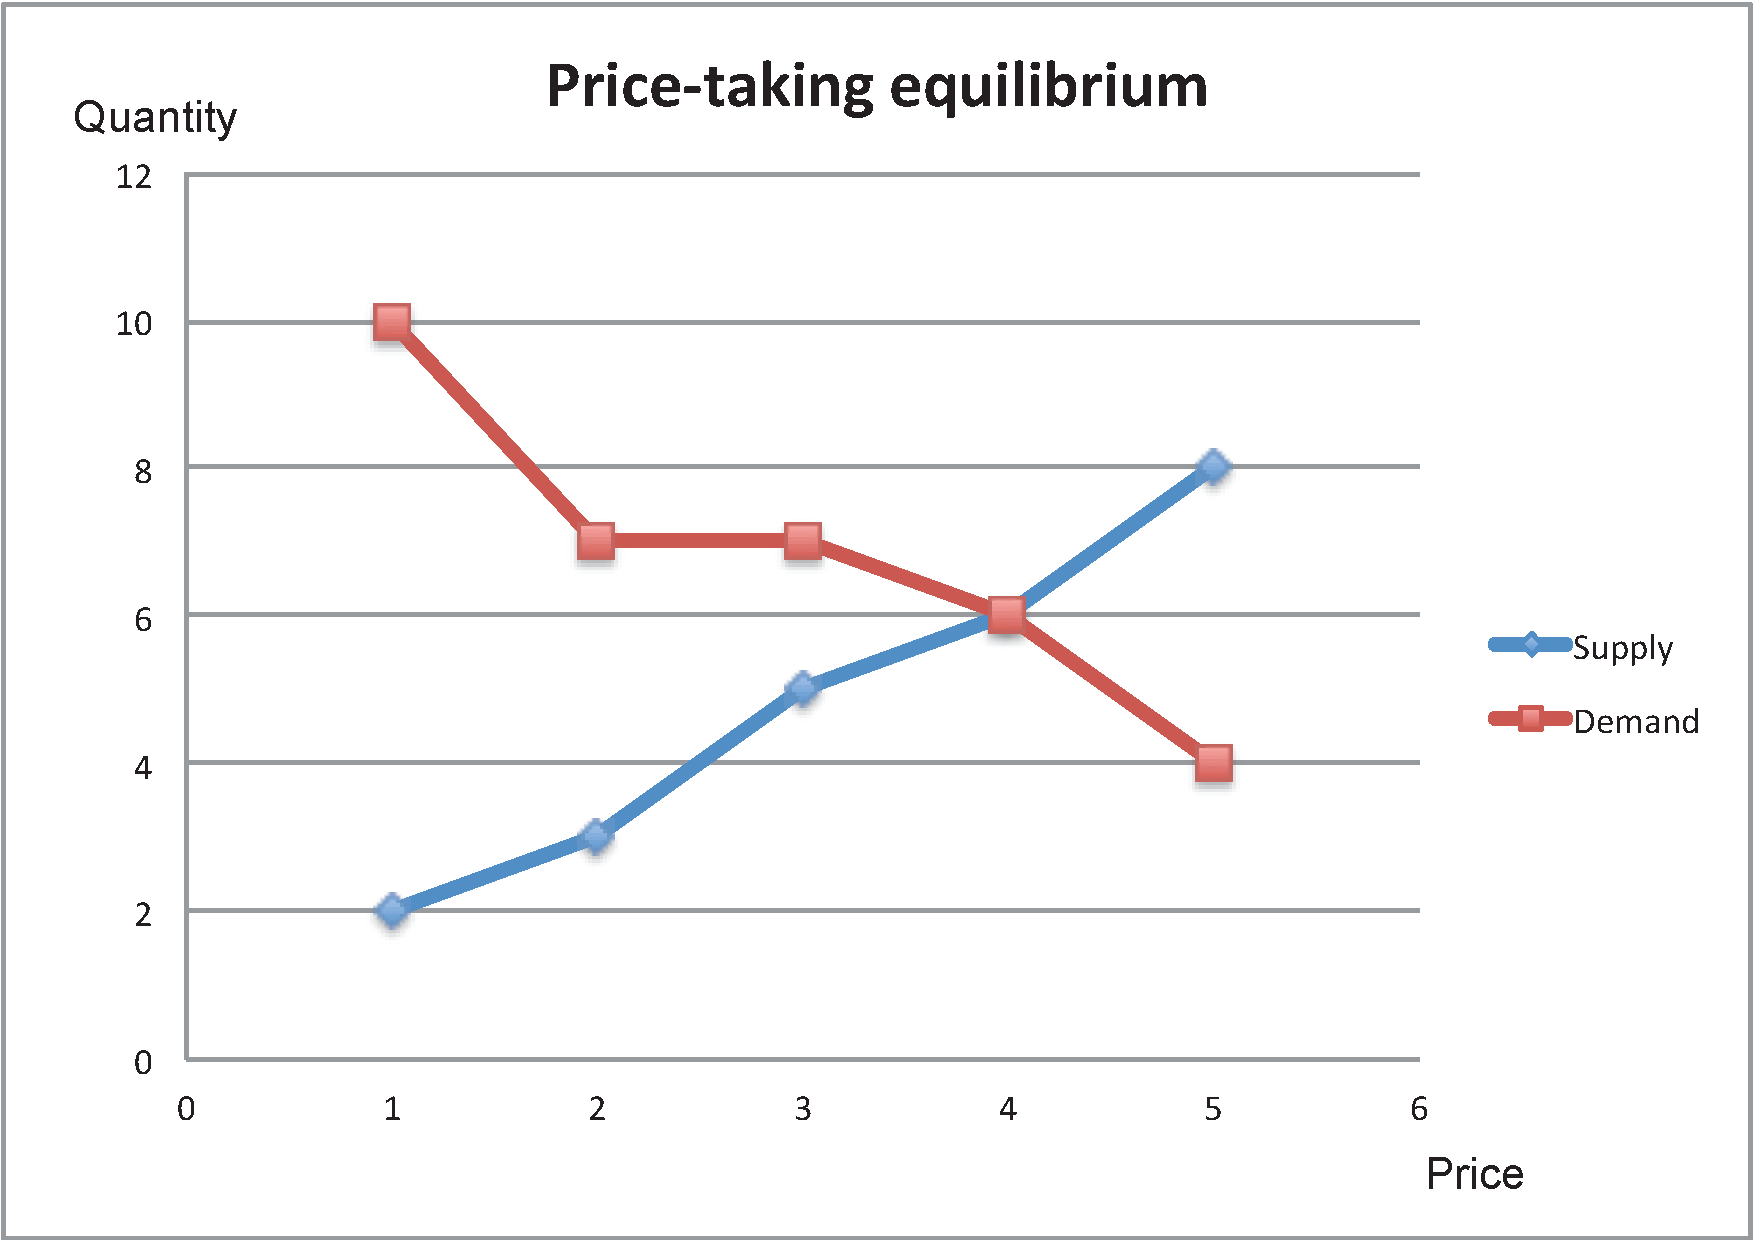
\includegraphics[width=.4\paperwidth]{pics/Image_PriceTaking2}
	\end{figure}
	Here: agents truthfully state their demand/supply
\end{frame}


\begin{frame}{Strategic bidding}
	\begin{itemize}
		\item What if agent 2 prefers 5 units at price 3 instead of 6 units at price 4?
		\item He can 'lie' about his demand schedule to the auctioneer
		\item Suppose he says he demands 10, 7, 5, 5, 4
	\end{itemize}
	\begin{figure}
		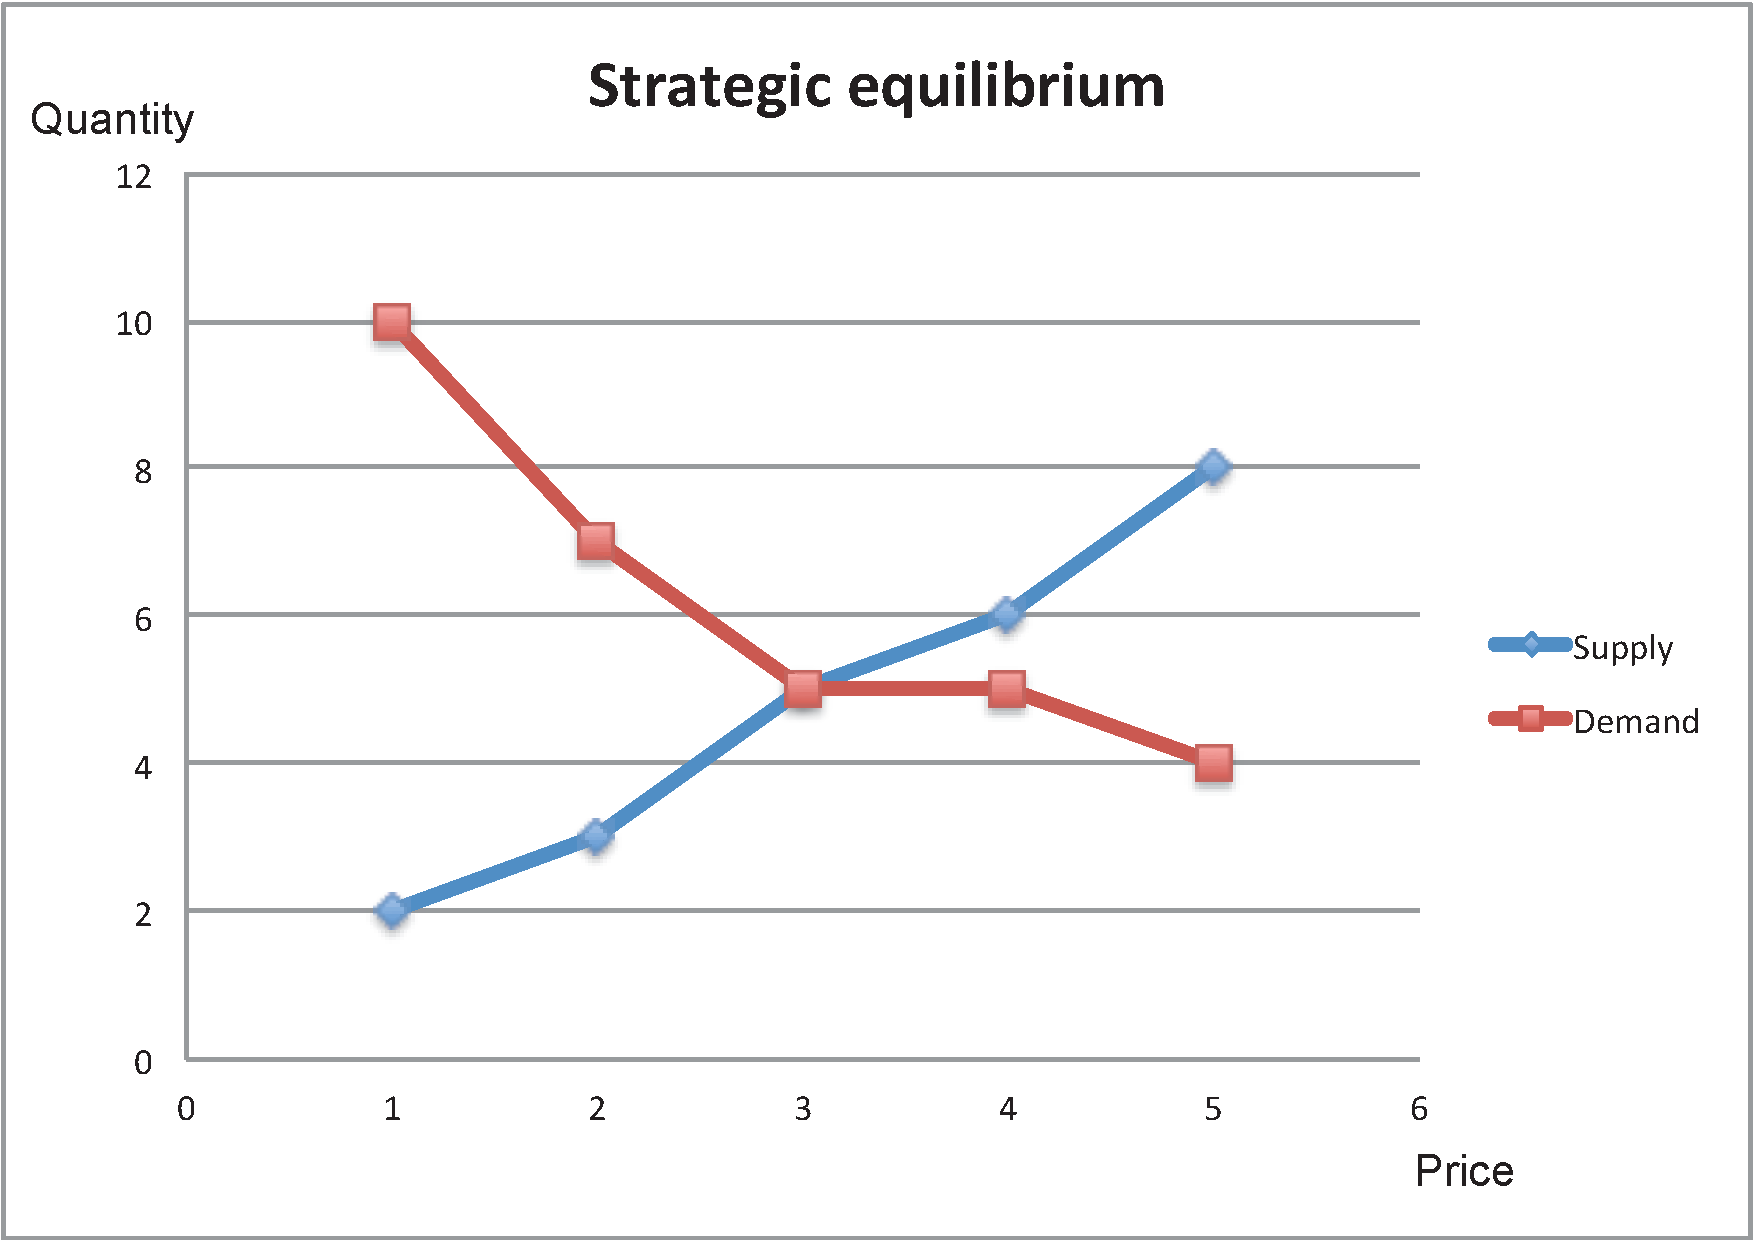
\includegraphics[width=.4\paperwidth]{pics/Image_Strategic2}
	\end{figure}
	Why would agent 2 want fewer units? Pay lower price on all units. (Parallel to monopolist restricting supply to get higher price). \hyperlink{main2}{\beamerbutton{back}}
\end{frame}



\end{document} 